\documentclass[tikz,border=10pt]{standalone}
\usepackage{tikz}
\usetikzlibrary{arrows.meta,arrows}
\usetikzlibrary{angles,quotes}
\usepackage{amsmath}
\usepackage{physics}

\ExplSyntaxOn
\msg_redirect_name:nnn { siunitx } { physics-pkg } { none }
\ExplSyntaxOff

\begin{document}
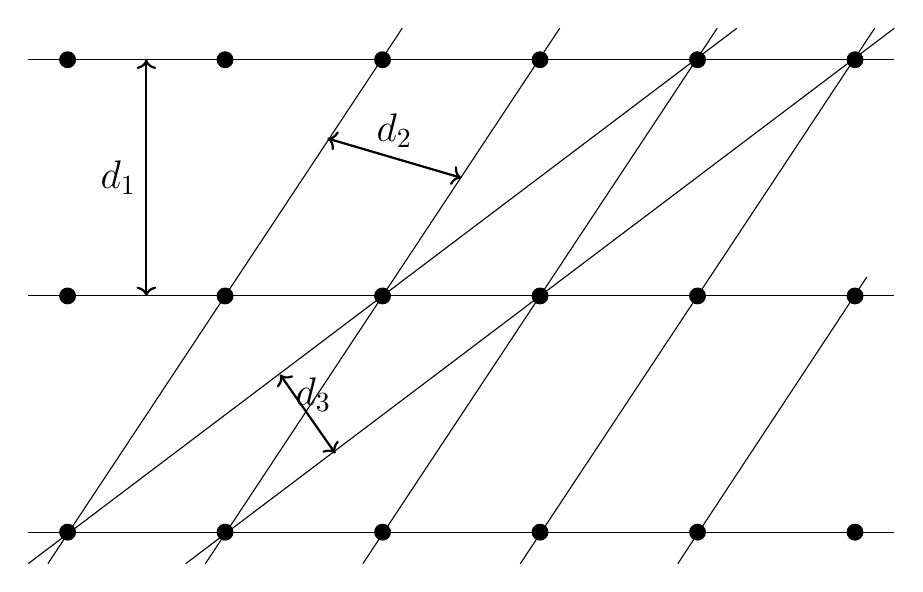
\begin{tikzpicture}[scale=2]
    \draw (-0.25, 0) -- (5.25, 0);
    \draw (-0.25, 1.5) -- (5.25, 1.5);
    \draw (-0.25, 3) -- (5.25, 3);

    \foreach \x in {0, 1, 2, 3, 4, 5}
    {
        \draw[fill] (\x, 0) circle (0.05);
        \draw[fill] (\x, 1.5) circle (0.05);
        \draw[fill] (\x, 3) circle (0.05);
    }

    \draw[-{Stealth[length=3mm, width=2mm]}, thick, <->] (0.5, 1.5) -- (0.5, 3) node[midway, left] {\Large{$d_{1}$}};

    \foreach \x in {0, 1, 2, 3}
        \draw (\x-0.125, -0.2) -- (\x+2.125, 3.2);
    
    \draw (3.875, -0.2) -- (5.075, 1.62);
    
    \foreach \x in {0, 1}
        \draw (\x-0.25, -0.2) -- (\x+4.25, 3.2);
    
    \draw[-{Stealth[length=3mm, width=2mm]}, thick, <->] (1.65, 2.5) -- (2.5, 2.25) node[midway, above] {\Large{$d_{2}$}};

    \draw[-{Stealth[length=3mm, width=2mm]}, thick, <->] (1.35, 1) -- (1.7, 0.5) node[pos=0.6, above] {\Large{$d_{3}$}};
\end{tikzpicture}
\end{document}